\documentclass[12pt]{article}
\usepackage{amsfonts, amssymb, amsmath, amsthm}
\usepackage[margin=1in]{geometry}
\usepackage{tikz}

\title{Explainer: Problem 4 (Rudin 7.1) --- Uniform Convergence $\Rightarrow$ Uniform Boundedness}
\author{}
\date{}

\begin{document}
\maketitle

\section*{What's being claimed?}
If $\{f_n\}$ is a sequence of bounded functions (each $|f_n(x)| \leq M_n$ for some constant $M_n$) and $f_n \to f$ \textbf{uniformly}, then there is a \emph{single} constant $M$ with $|f_n(x)| \leq M$ for \emph{all} $n$ and \emph{all} $x$.

\section*{Two kinds of boundedness}
\begin{itemize}
  \item Each $f_n$ bounded: for each $n$, some $M_n$ works. But $M_n$ could blow up in $n$.
  \item \textbf{Uniformly bounded:} one single $M$ works for the whole sequence.
\end{itemize}

\section*{Why uniform convergence helps}
Uniform convergence means: eventually, \emph{all} $f_n$ are within $\varepsilon$ of $f$ \emph{everywhere}. Once you're close to $f$, you inherit $f$'s bound. The only worry is the finitely many terms \emph{before} that point --- but finitely many bounded functions are jointly bounded (take the max).

\begin{center}
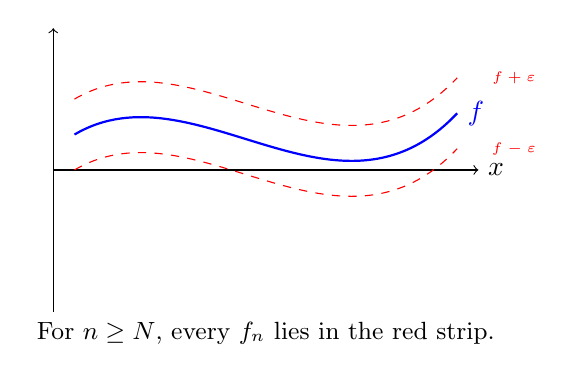
\begin{tikzpicture}[scale=0.9]
  \draw[->] (0,0) -- (6,0) node[right] {$x$};
  \draw[->] (0,-2) -- (0,2);
  \draw[thick, blue] (0.3, 0.5) .. controls (2, 1.5) and (4, -1) .. (5.7, 0.8) node[right] {$f$};
  \draw[dashed, red] (0.3, 1) .. controls (2, 2) and (4, -0.5) .. (5.7, 1.3);
  \draw[dashed, red] (0.3, 0) .. controls (2, 1) and (4, -1.5) .. (5.7, 0.3);
  \node[red] at (6.5, 1.3) {\tiny $f+\varepsilon$};
  \node[red] at (6.5, 0.3) {\tiny $f-\varepsilon$};
  \node at (3, -2.3) {\small For $n \geq N$, every $f_n$ lies in the red strip.};
\end{tikzpicture}
\end{center}

\section*{Strategy}
\begin{enumerate}
  \item Use uniform convergence: pick $N$ so that $|f_n(x) - f(x)| < 1$ (any $\varepsilon$) for all $n \geq N$ and all $x$.
  \item $f$ is bounded (as a uniform limit of bounded functions --- prove this first!).
  \item For $n \geq N$: $|f_n(x)| \leq |f(x)| + 1 \leq \|f\|_\infty + 1$.
  \item For $n < N$: just finitely many; each has its own bound $M_n$.
  \item Take $M = \max(M_1, \ldots, M_{N-1}, \|f\|_\infty + 1)$.
\end{enumerate}

\section*{A subtle step: the limit is bounded}
You'll need $|f(x)| \leq \|f_N\|_\infty + \varepsilon$ for all $x$, which follows from $|f(x) - f_N(x)| < \varepsilon$ and $|f_N(x)| \leq \|f_N\|_\infty$.

\end{document}
